\section{Formative Study}
We conduct a formative study to inform the design of our approach. First, to understand the core process of GraphRAG, we surveyed existing papers and high-impact open-source projects involving GraphRAG. Based on the survey, an abstraction of the common pipeline of GraphRAG is summarized in Section \ref{Common Architecture of GraphRAG}. Second, we conducted a formative interview with 5 RAG experts to identify the challenges encountered during the analysis of the GraphRAG process with existing tools in Section \ref{Common Architecture of GraphRAG}. Finally, we distill the four design requirements to improve the analysis process.

\subsection{Common Pipeline of GraphRAG}
\label{Common Architecture of GraphRAG}

\begin{figure}[htb]
    \centering
    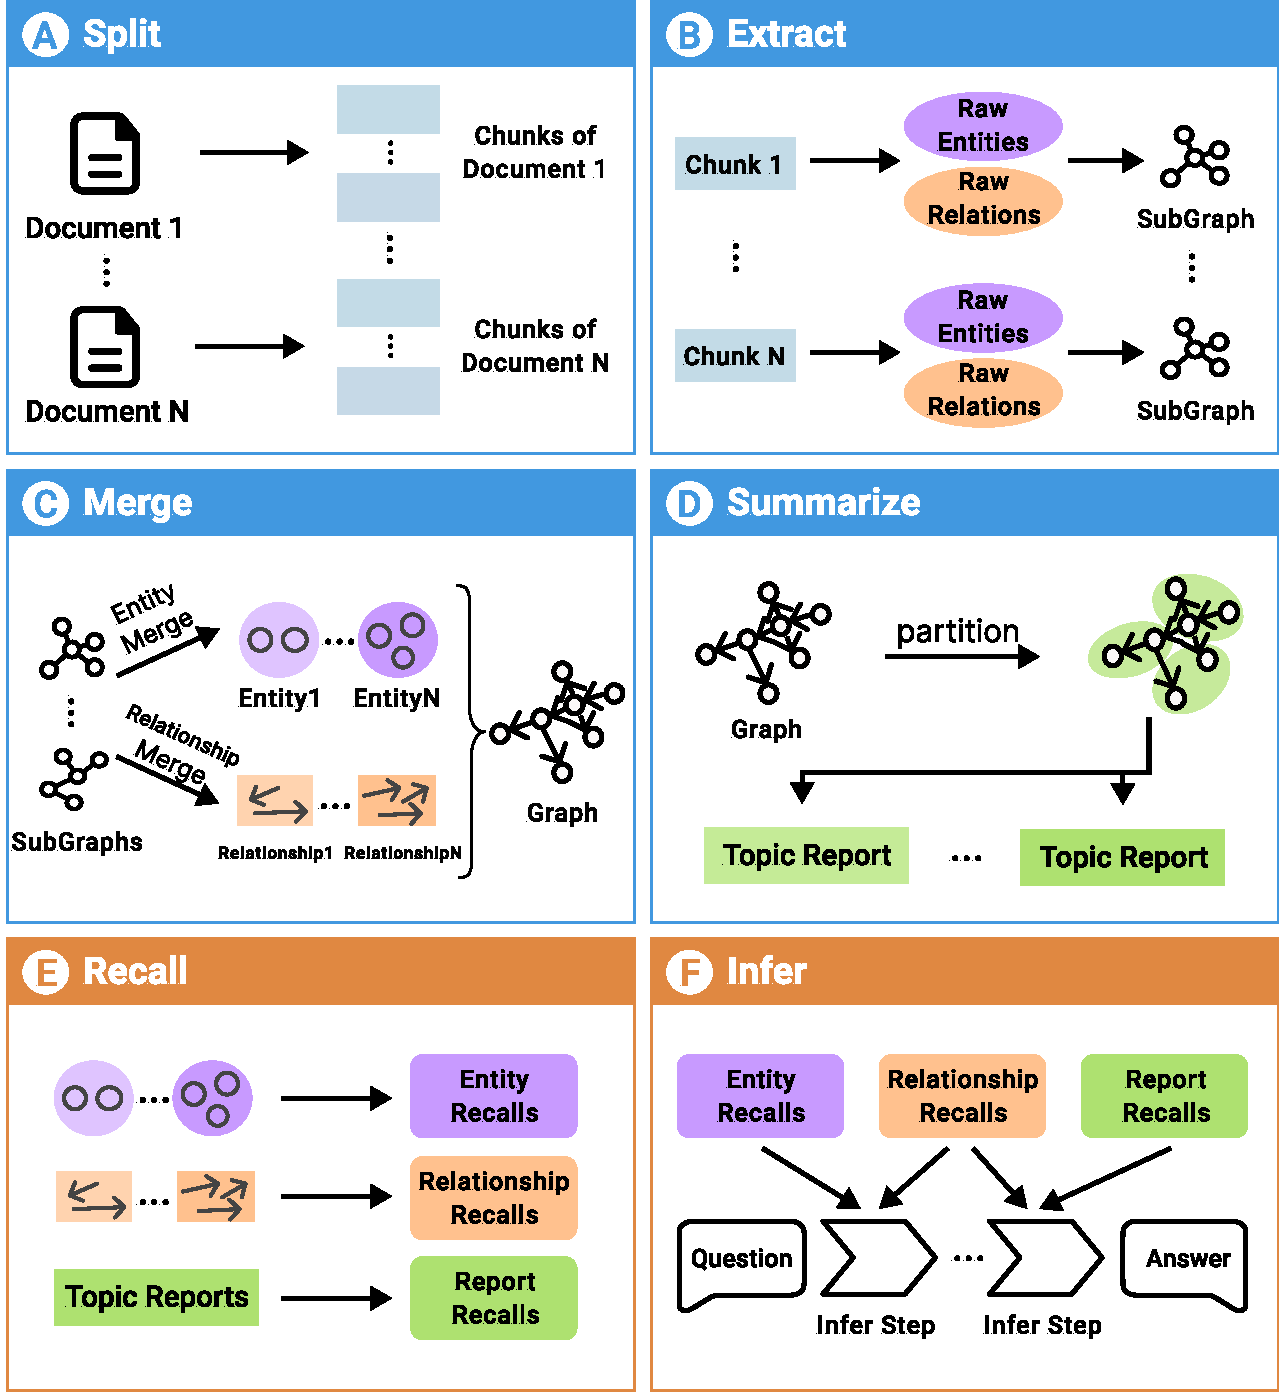
\includegraphics[width=\linewidth]{figs/CommonArchitecture.pdf} % 图片文件名
    \caption{Common Pipeline of GraphRAG, which is typically divided into an offline construction phase (a-d) and an online retrieval phase (e-f).} % 图片说明
    \label{fig:common-architecture} % 图片标签
  \vspace{-10pt}
    
\end{figure}

We survey recent GraphRAG-related papers and open-source projects to abstract the typical components of a GraphRAG pipeline. Given that GraphRAG is an emerging field with many works still awaiting peer review, we identified influential papers/projects in this area based on recommendations from RAG experts and search terms ``GraphRAG'', ``Graph Retrieval Augmented Generation'', ``Knowledge Graph RAG'', ``Graph-based RAG'', and ``Graph-augmented LLM''. Starting with several influential seeding works (e.g., GraphRAG\cite{edge2024local}, KAG\cite{liang2024kag}, LightRAG\cite{guo2024lightrag}), we iteratively expanded our corpus by analyzing both the references within these works and the works that cite them. Our final collection comprises 30 GraphRAG-related works (list included in our supplementary materials). Drawing from this corpus, we analyzed and summarized the essential data elements and data processing components shared by them. As shown in Fig~\ref{fig:common-architecture}, the GraphRAG pipeline is typically divided into two main components: an offline construction phase (a-d) and an online retrieval phase (e-f). We elaborate on the essential data process stages for each phase as follows.


\subsubsection{Construction Phase}
\label{Construction Phase}

\textbf{Split:} The initial step involves dividing the original documents into smaller, manageable \textbf{text chunks}. This segmentation is crucial as it sets the foundation for subsequent processing. The text chunks are designed to be coherent units of information, facilitating easier extraction and analysis in later stages.

\textbf{Extract:} For each text chunk, we extract \textbf{raw entities} and \textbf{raw relationships}, forming \textbf{subgraphs}. This involves identifying key elements within the text, such as names, dates, and specific terms, and understanding how these elements relate to each other. Each entity and relationship is enriched with additional metadata, such as \textbf{descriptions} and \textbf{entity types}, which provide context and clarity, enhancing the granularity of the subgraphs.

\textbf{Merge:} The next step is to combine these subgraphs into a comprehensive \textbf{graph}. This involves resolving conflicts where entities and relationships share names but differ in context. The merging process ensures that information is unified, with \textbf{entity} and \textbf{relationship} descriptions being consolidated. This step is critical for maintaining data integrity and ensuring that the graph accurately reflects the source material. Each \textbf{node} and \textbf{edge} in the graph is annotated with \textbf{chunk references} to the original text chunks from which they were derived, ensuring traceability.

\textbf{Summarize:} Once the graph is complete, it is partitioned based on the density of relationships among entities, resulting in distinct \textbf{topics}. This partitioning helps in organizing the graph into meaningful segments, each representing a coherent topic or theme. Within each topic, the entities and relationships are summarized to create concise \textbf{reports}. These summaries are constructed with clear references to the specific entities and relationships they are derived from, ensuring transparency. Depending on the complexity of the original corpus and the graph, this partitioning may occur at multiple hierarchical levels, providing varying degrees of abstraction and detail.

Throughout the construction phase, large language model invocations are extensively employed at different stages for natural language processing tasks. These models assist in tasks such as entity recognition, relationship extraction, and summarization, leveraging their advanced capabilities to enhance the accuracy and efficiency of the process.

\subsubsection{Retrieval Phase}

\textbf{Recall:} During the retrieval phase, user \textbf{queries} are utilized to extract relevant information from the constructed graph. The system identifies and retrieves various types of \textbf{recalls}, such as \textbf{entity recalls}, \textbf{relationship recalls}, and \textbf{report recalls}. This involves searching the graph for nodes and edges that are relevant to the user's query, ensuring that the most pertinent information is brought to the forefront.

\textbf{Infer:} The LLM then uses these recalls to perform step-by-step \textbf{inference}. Each inference step is explicitly linked to specific recalls, ensuring that the reasoning process is transparent and traceable. This iterative process allows the system to build upon retrieved information, synthesizing it to generate comprehensive answers. The inference culminates in producing a final \textbf{response} to the user's query, leveraging the depth and breadth of the graph's information.

This structured approach enhances the GraphRAG system's ability to manage and utilize complex relationships within data, supporting more effective retrieval and reasoning capabilities. By providing clear traceability and leveraging advanced language models, the system ensures both accuracy and transparency in its responses.

\subsection{Challenges of Analyzing the GraphRAG Process}
\textbf{Participants and procedure.} To understand the challenges users could encounter during the analysis of the GraphRAG process, we conducted a formative interview with 5 RAG experts. Three of them (E1-E3) are experienced RAG engineers who have first-hand experience with GraphRAG in their projects. The other two (E4-E5) are RAG researchers who have conducted at least one GraphRAG-related research project. In our interview, we first asked the participants about their current workflow for analyzing the GraphRAG process on their datasets and the challenges they encountered during this process. After that, we showed them how to use \textit{Kotaemon} \cite{kotaemon}, one of the most popular open-source projects that provide interactive analysis support for the GraphRAG process. We then asked the participants to try out \textit{Kotaemon} on their own in a think-aloud way (reporting the analysis target and the challenges they encountered in situ). We also collected participants' overall feedback at the end of the interview. Based on the interview, we summarize the challenges as follows.

\textbf{Lack of traceability across the complex information processing pipeline.} All of the participants mentioned the necessity and difficulty of tracing through the information processing pipeline of GraphRAG. To analyze the cause of the final or intermediate output, the participants need to "examine its upstream modules step by step" (E2). Nevertheless, this demand is not well-supported by existing tools. \textit{Kotaemon} \cite{kotaemon} provides some support for certain steps (e.g. users can click an entity to trace the chunk it is extracted from), but "lacks complete traceability from the final answer back to the raw document chunks" (E1).

\textbf{Lack of revealing of LLM invocation context on the graph.} The GraphRAG process typically involves hundreds or even thousands of LLM invocations to construct and query the graph. The participants mentioned that they often feel "overwhelmed and lost in the sea of LLM calls" (E2) and "hard to connect certain LLM invocation with its specific role on graph" (E5). Existing tools only provide exclusive or separate support for graph analysis for LLM invocation analysis. However, it is highly desirable to provide support for "analyzing LLM invocations on the graph" (E4). 

\textbf{Lack of support for multi-facet relevance analysis on the graph.} The key to the success of GraphRAG lies in whether it can utilize the graph structure to capture the relevance between the information in the customized corpus and the user's query. This relevance can be explicit local connectivity on the graph, or semantic connectivity based on global structure and specific techniques applied for graph summarization (as discussed in Section \ref{Construction Phase}). However, there is a lack of support for systematic analysis of different types of relevance on the graph. As E2 mentioned, "the key lies in finding why some relevance is successfully or unsuccessfully captured and exploited on graphs, which is a very complex and demanding analysis process"

\subsection{Design Requirement}

In response to the challenges identified in our formative study, we aim to design a visual analysis system to facilitate the analysis process for GraphRAG. The design requirements are distilled as follows:

\textbf{R1: Facilitate step-by-step trace for the generated answer.} To understand the final or intermediate output, users need to trace back to its upstream modules step by step. This traceability ensures that users can verify the accuracy of each step and identify the root cause of unexpected results. The system should provide flexible interaction and visualization to facilitate this tracing process.

\textbf{R2: Reveal LLM invocation context on the graph.} There is a large quantity of LLM invocations during the GraphRAG process. While those LLM invocations play a vital role in information extraction and processing during graph construction and query, it is hard for analyzers to link each invocation with its context on the graph during the analysis process. Therefore, it is highly desirable to provide support to help users understand the structure and context of those invocations.

\textbf{R3: Support global relevance analysis on the graph.} A significant advantage of GraphRAG over conventional RAG is its ability to use graphs to capture global semantic information. For example, if certain entities are not directly connected but are frequently mentioned in the context of certain topics, they might be grouped into the same community by GraphRAG, which is essential for answering questions that require a broader, more holistic understanding. Therefore, analysis support for the underlying process is important for understanding why GraphRAG succeeds or fails in different settings.

\textbf{R4: Support local relevance analysis on the graph.} While GraphRAG excels at capturing global semantic information, it also greatly enhances recall quality by leveraging local graph connectivity to capture local relevance. For instance, if a user's query pertains to a particular entity, understanding the direct connections and relationships of that entity can provide more precise and contextually relevant answers. Therefore, it is also important to provide support for a detailed, localized analysis of the graph.